\section{laying pipes in the clouds}\label{sec:rate-control}

\subsection{The Dream Network Pipe}\label{subsec:dream-pipe}

\begin{figure*}[!t]
  \centering
    \begin{subfigure}{0.65\columnwidth}
  \centering
  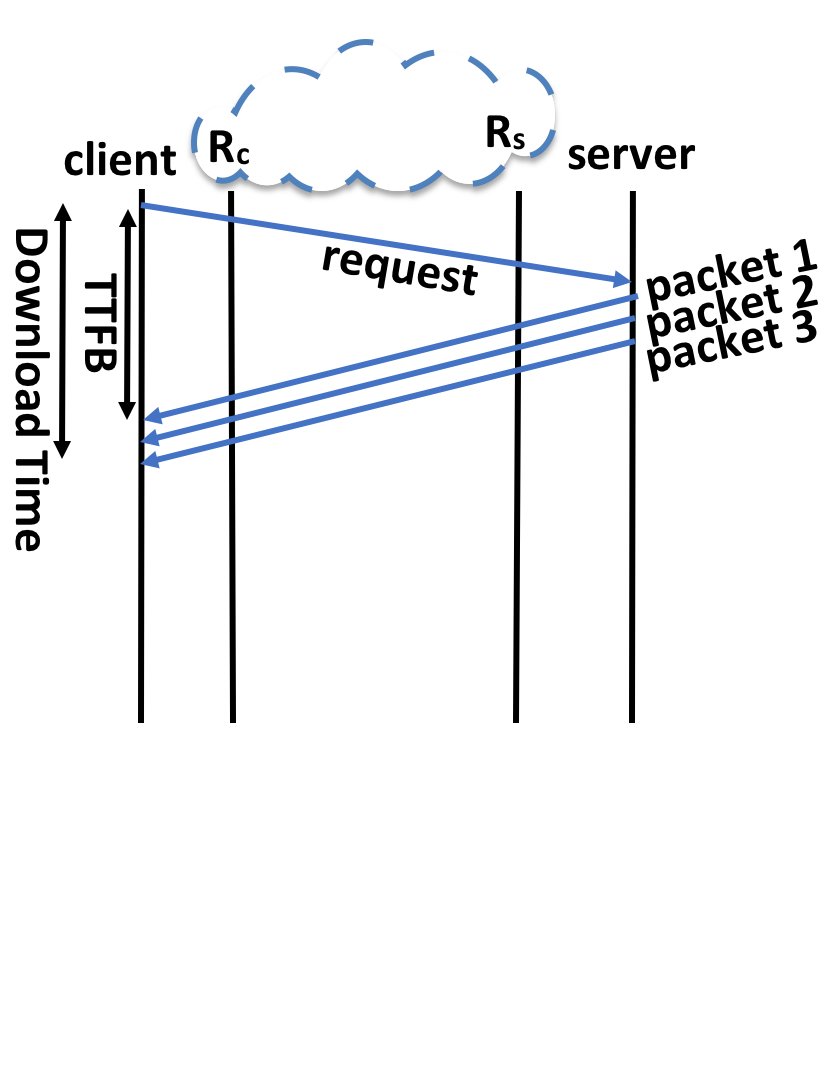
\includegraphics[width=\columnwidth]{figures/ideal.png}
    \caption{Ideal protocol-free transmission.}
    \label{fig:ideal}
\end{subfigure}    \centering
\begin{subfigure}{0.65\columnwidth}
  \centering
  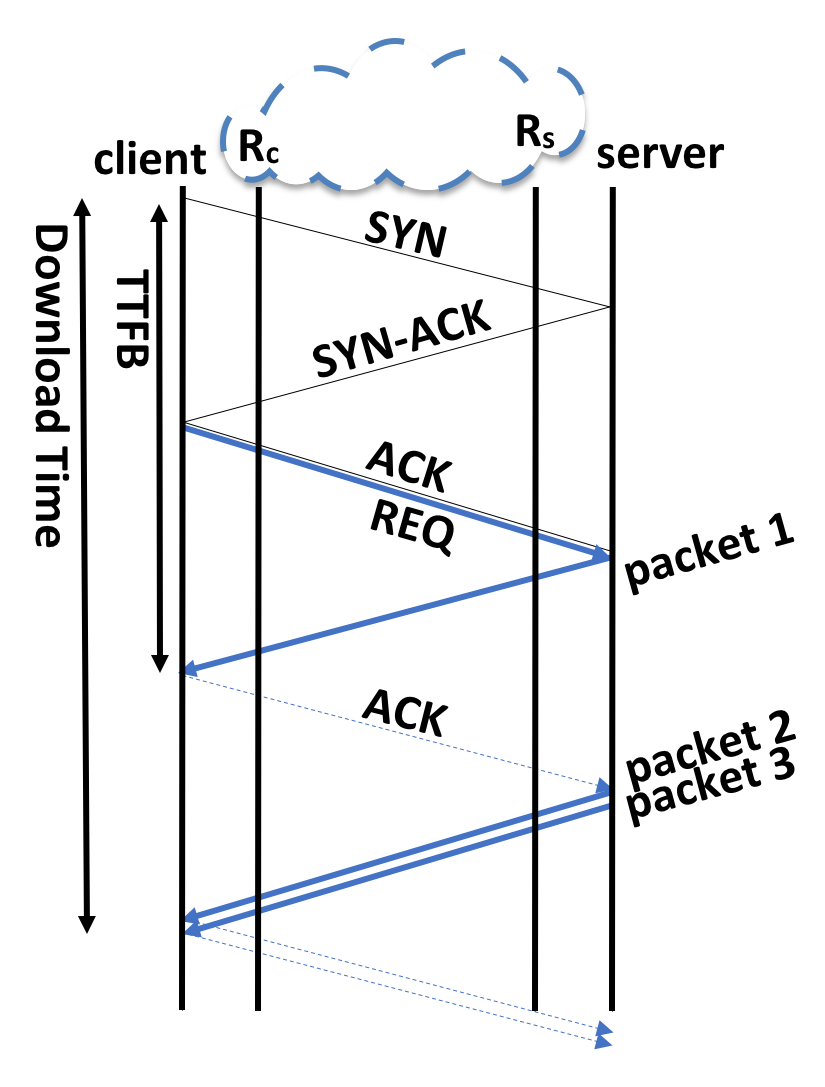
\includegraphics[width=\columnwidth]{figures/e2e.png}%test1.pdf}
    \caption{End-to-end through the Internet (or cloud).} \label{fig:e2e}
\end{subfigure}    \centering
\begin{subfigure}{0.65\columnwidth}
  \centering
  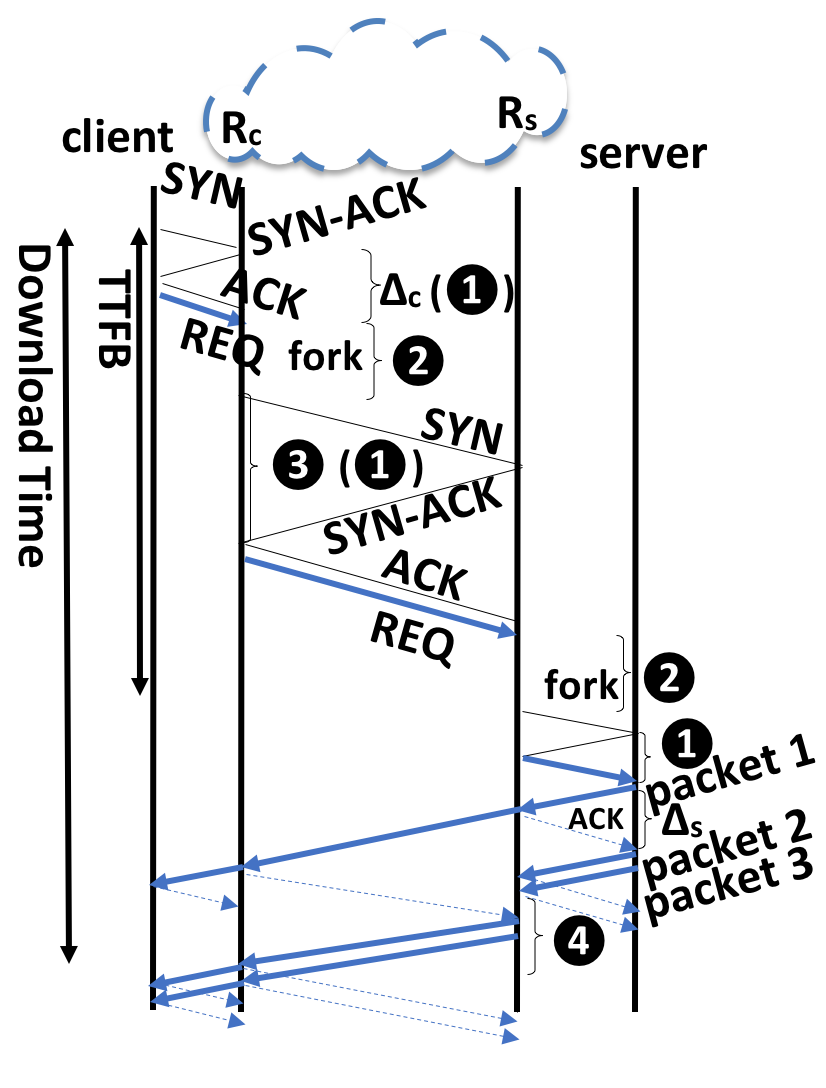
\includegraphics[width=\columnwidth,clip]{figures/split.png}
    \caption{Simple TCP cloud split.} \label{fig:baseline}
\end{subfigure}
%  \centering
% \begin{subfigure}{0.6\columnwidth}
%   \centering
%   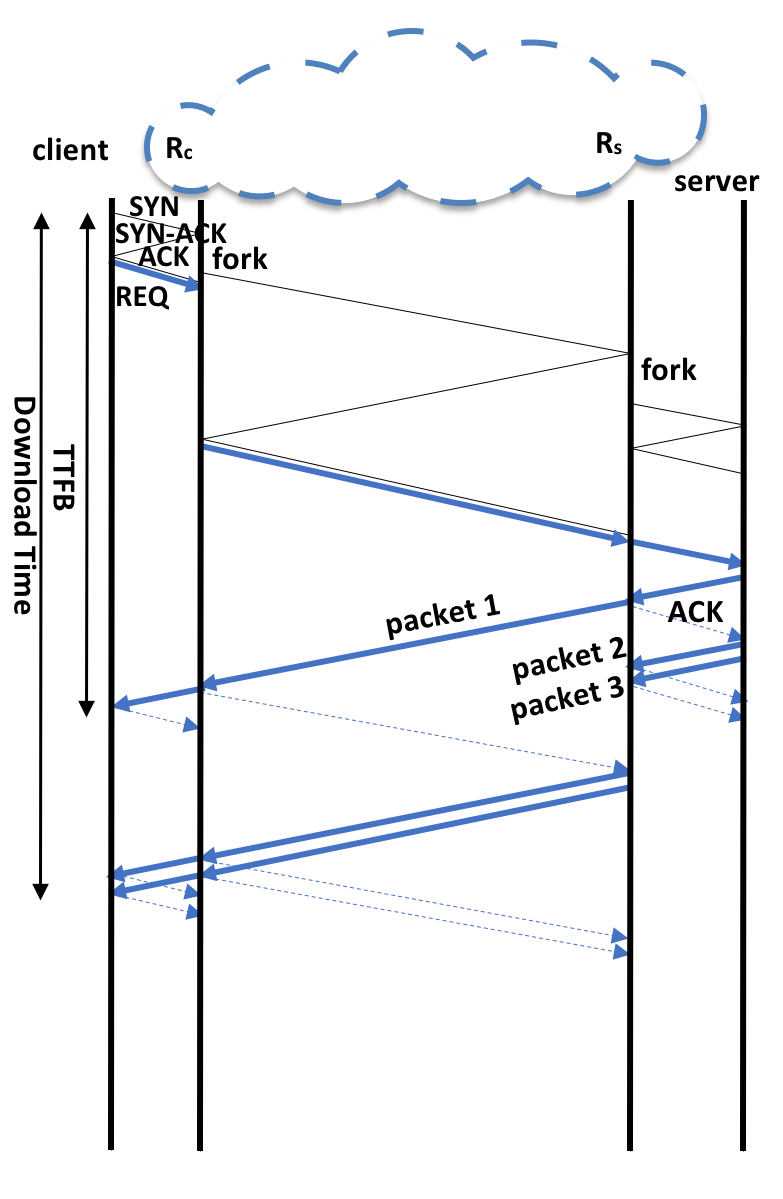
\includegraphics[width=\columnwidth]{figures/early-syn.png}
%     \caption{Early-SYN.} \label{fig:early-syn}
% \end{subfigure}
    \caption{Illustrated comparison of the considered baseline data transmission methods. Suppose, for simplicity of exposition, that the client requests three MSS-sized packets using HTTP over TCP, that the initial TCP window size is one MSS, and that there are no losses.\\ \textit{(a)} In an ideal clean-slate world, the request for packets would go through directly, triggering the transmission of all response packets. The time-to-first-byte (TTFB) is just one round-trip time (RTT), the lowest possible TTFB. The download time is barely higher.\\ \textit{(b)} End-to-end TCP transmission first requires the establishment of an end-to-end connection, adding one RTT to the ideal finish time. Waiting one RTT for the first ACK further delays the download. \\ \textit{(c)} The baseline strategy of Section~\ref{sec:ocd-baseline} decreases the ACK times for longer files, but introduces new delays such as thread fork delays in the connection. This explains why the Baseline is less efficient for small files. We later revisit all the delays that appear beyond those of the ideal transmission (Figure~\ref{fig:oursys-improvements}). We show how to address the delays marked (1)-(4), but are left with delays $\Delta_c$ and $\Delta_s$ on the client and server sides, respectively.  }
\end{figure*}

\begin{figure*}[!t]
  \centering
    \begin{subfigure}{0.48\columnwidth}
  \centering
  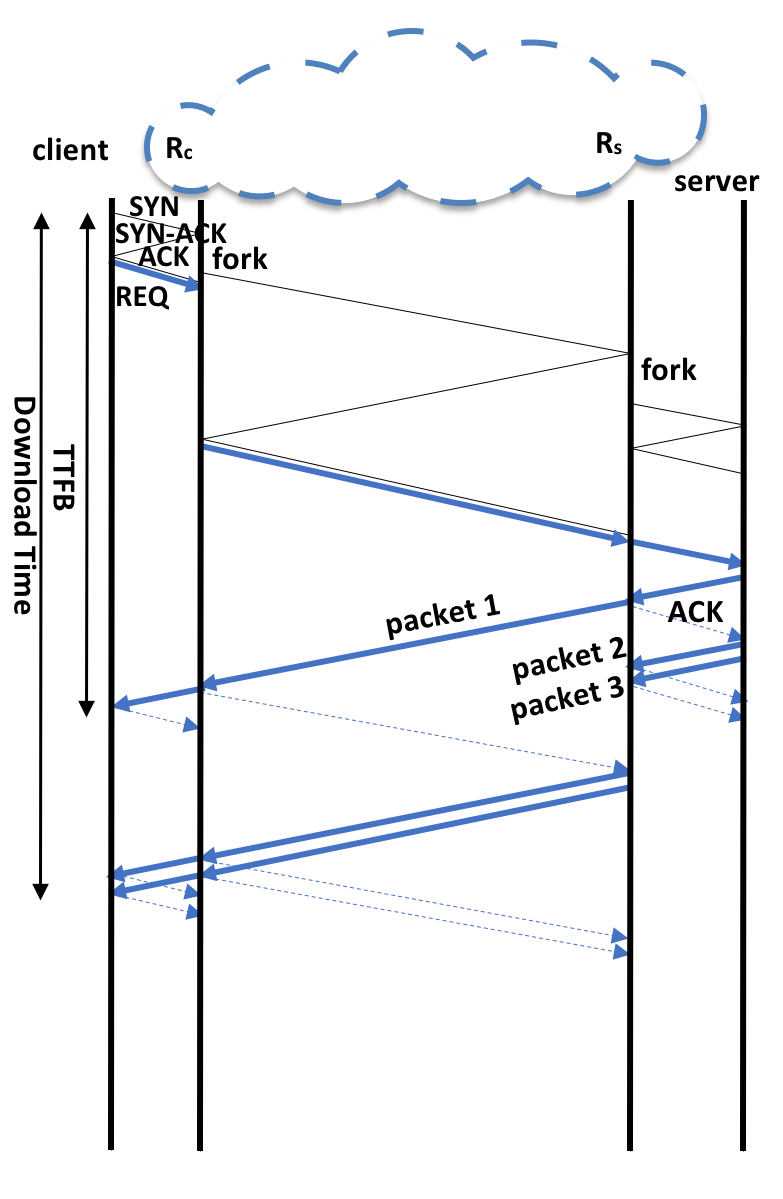
\includegraphics[width=\columnwidth]{figures/early-syn.png}
    \caption{Early-SYN.}
    \label{fig:early-syn}
\end{subfigure}    \centering
\begin{subfigure}{0.48\columnwidth}
  \centering
  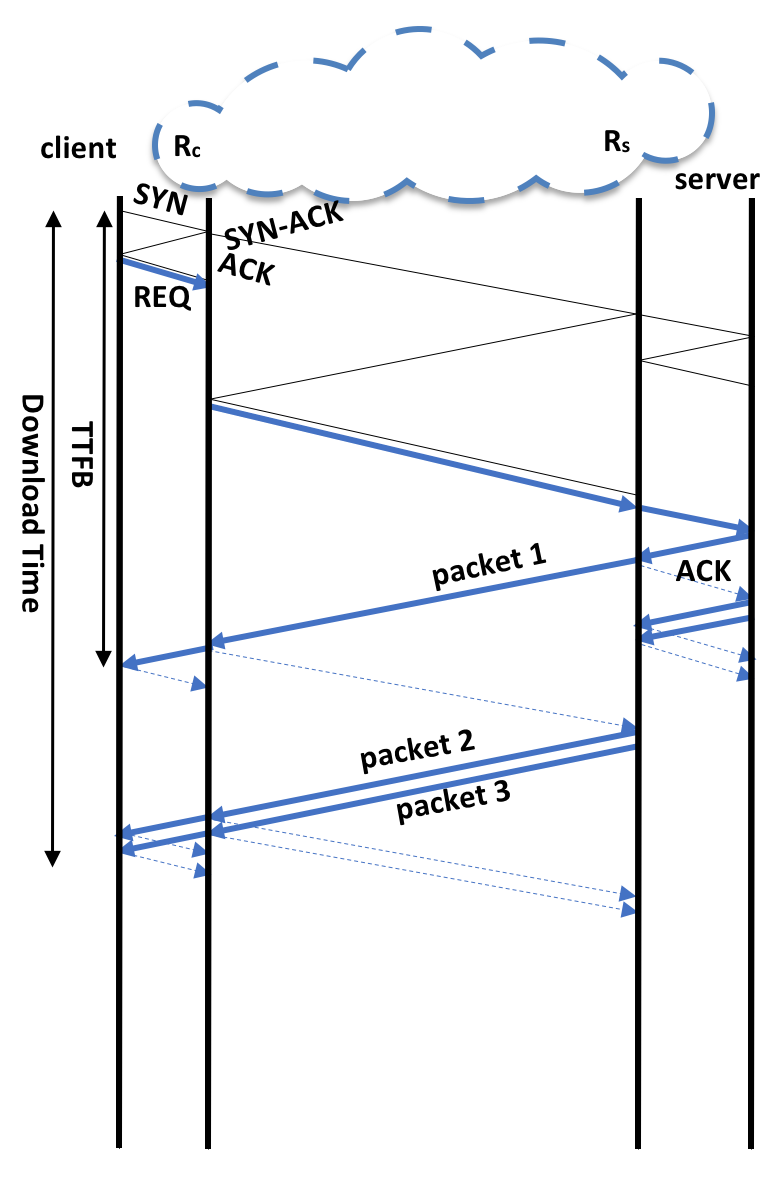
\includegraphics[width=\columnwidth]{figures/thread.png}
    \caption{Thread pool.} \label{fig:thread-pool}
\end{subfigure}    \centering
\begin{subfigure}{0.48\columnwidth}
  \centering
  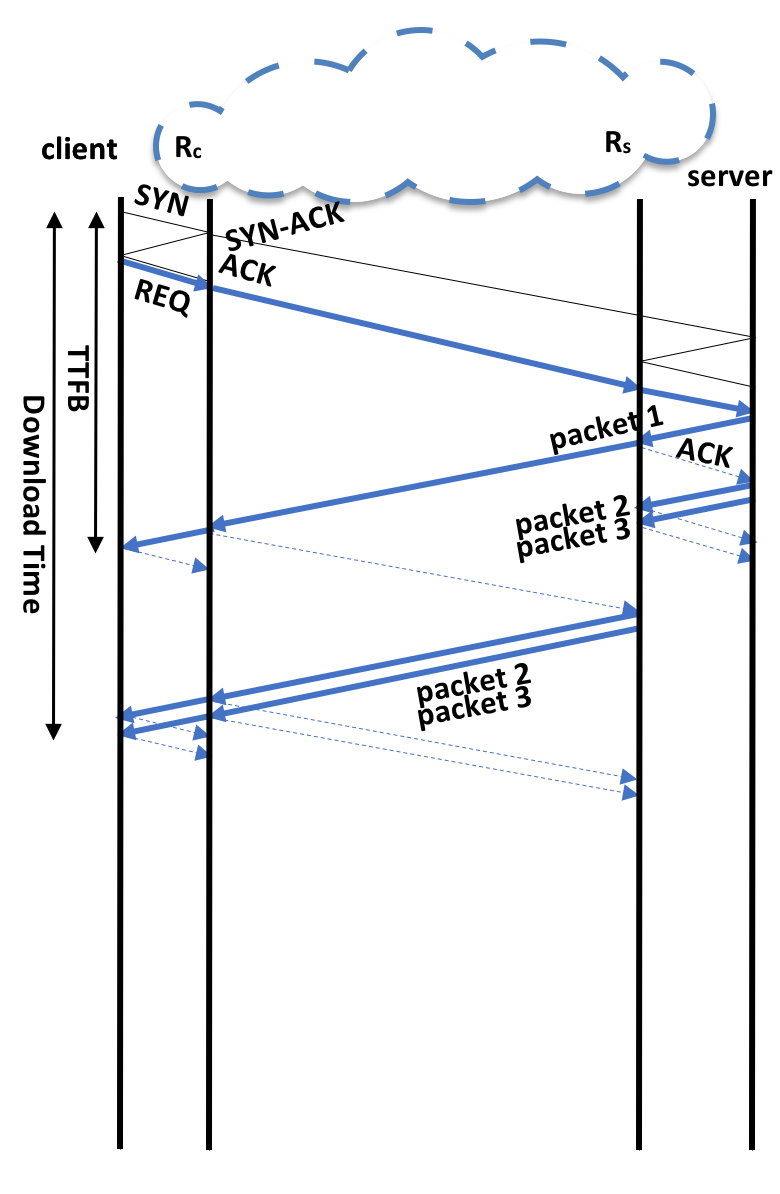
\includegraphics[width=\columnwidth]{figures/connection.png}
    \caption{Connection pool.} \label{fig:connection-pool}
\end{subfigure}     \centering
\begin{subfigure}{0.48\columnwidth}
  \centering
  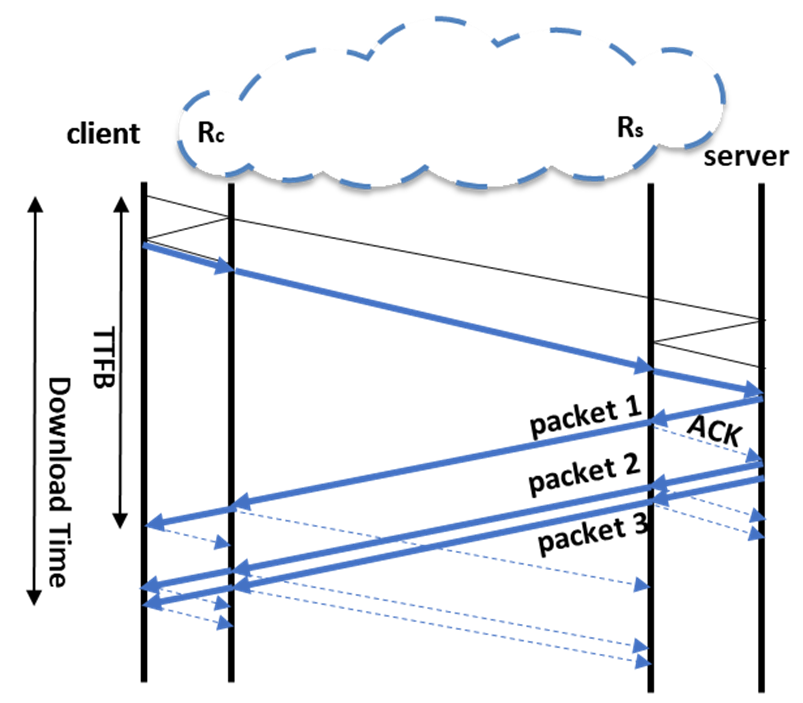
\includegraphics[width=\columnwidth]{figures/turbo.png}
    \caption{Turbo-Start TCP.} \label{fig:turbo-start-tcp}
\end{subfigure}
%  \centering
% \begin{subfigure}{0.6\columnwidth}
%   \centering
%   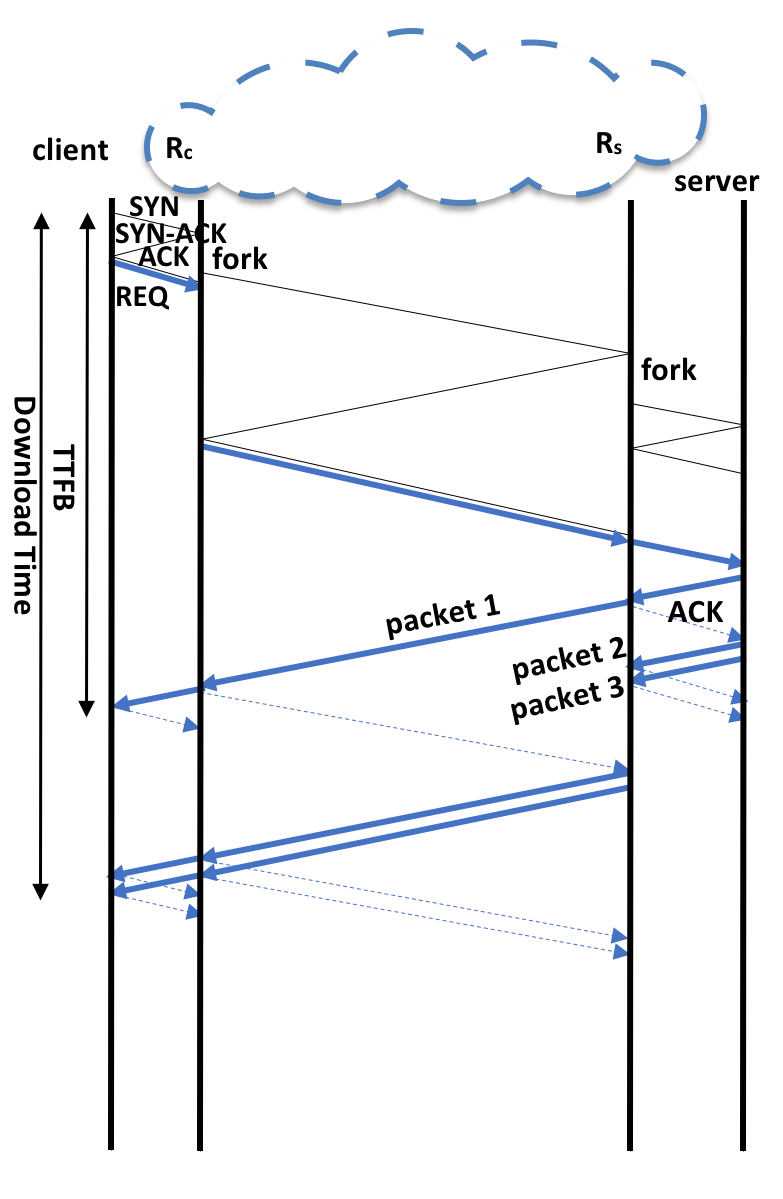
\includegraphics[width=\columnwidth]{figures/early-syn.png}
%     \caption{Early-SYN.} \label{fig:early-syn}
% \end{subfigure}
    \caption{\oursys successive implementation improvements: Using \textit{Early-SYN}, we can remove SYN-ACK and ACK delays (marked as (1) in Figure~\ref{fig:baseline}). Using a \textit{thread pool} removes forks (marked as (2) in Figure~\ref{fig:baseline}). With a \textit{connection pool}, delay (3) in Figure~\ref{fig:baseline} is eliminated. Turbo-Start TCP eliminates delay (4). The two last delays (marked as ``?'' in Figure~\ref{fig:baseline}) that need be removed are delays $\Delta_c$ and $\Delta_s$ on the client and server sides, respectively. As both depend on the client and server parameters, they seem beyond our control. 
    }
    \label{fig:oursys-improvements}
\end{figure*}

%\T{Congestion-less control?} The cloud provides an auto-scaling networking infrastructure with links of virtually-infinite capacity. Like others~\cite{haq2017measuring}, we find that in-cloud paths provide more predictable results than the public Internet, with an order of magnitude lower loss rate. As a result, flows in the cloud will rarely ever encounter congestion. This compels us to rethink the role of congestion control in the cloud. In light of the near-absence of congestion, we essentially want a simple high-rate sending protocol capable of dealing with the very rare loss events, without necessarily backing off. Even flow control is not necessarily needed within the cloud, as clouds can increasingly provide an elastic memory infrastructure~\cite{hotadd,baloon} that can quickly adapt to any receive-buffer temporary load. 

\T{Ideal pipe.} Given the large capacity of the cloud, we wonder how close we could get to an ideal transmissio..
\autoref{fig:ideal} illustrates our fundamental model of an ideal transmission. Importantly, this model reflects a protocol-free, theoretical ideal transmission. Our aim for the remainder of this section is to identify the means for approximating this model in practice. We show in \autoref{fig:e2e} that a classical end-to-end data transfer based on HTTP over TCP falls short 
%\AB{I'm not sure how CC got into this... Some of the delays are not due to congestion control, but due to TCP's operation and design tradeoffs, regardless of CC. Also, should we mention that the diagram assumes HTTP as the transport protocol? (Does it also fit others, like, \eg FTP?)} congestion control falls short 
of this goal. In addition, adding a stop on our  also introduces additional delays with respect to the ideal model. We point out these delays in \autoref{fig:baseline}, and discuss how these delays can be eliminated, so as to come close to our theoretical ideal.

%Realizing rate-control for the cloud could have simply utilized a form of Reliable UDP. To be backwards compatible, we simply used instead a Cubic TCP with an aggressive initial window size.

\subsection{Approximating the Ideal Pipe}\label{sec:approx}

To approximate the ideal data transmission model of Section~\ref{subsec:dream-pipe}, we introduce \textit{\oursys}.
The goal of \oursys is to enhance the OCD Baseline of Section~\ref{sec:ocd-baseline} and provide efficient, delay-free TCP optimization; while utilizing commodity VMs and standard programming APIs. This is done by incorporating four improvements to the baseline strategy, illustrated in Figure~\ref{fig:oursys-improvements}. Together, these four components eliminate the delays marked (1)-(4) in Figure~\ref{fig:baseline}. We next elaborate on each of the four improvements. We discuss the many implementation details involved in realizing \oursys in Section~\ref{sec:design} and provide our open-source code in~\cite{ktcp}.

%\oursys incorporates four improvements to the baseline strategy of Section~\ref{x}, illustrated in Figure~\ref{fig:baseline}. Together, these four improvements eliminate the delays marked (1)-(4) in \ref{fig:oursys-improvements}. We next elaborate on each of the four improvements. We discuss the many implementation details involved in realizing \oursys in Section~\ref{sec:design}.

%\AB{we need to change the order here. Perhaps also in the figure. The Early SYN (named Early SYN Forwarding (ESF) in earlier papers) option cannot be tested on its own, currently (Alex can explain). The first optimization is thread pool, then adding ESF and then changing adding the pre-existing connections...}\IK{Two isues: 1. Noga needs to redo the plots (=numbers in 5c+ full 6a); 2. Early-SYN was done in the past, the other 3 improvements were not, so this order is more logical in this sense...\\ ... that being said, if you/Noga/Eyal are willing to redo the graphs, feel free to go ahead.}


\T{Improvement 1: Early SYN.} In early SYN~\cite{ladiwala,siracusano2016miniproxy}, a SYN packet is sent to the next-hop server as soon as the SYN packet arrives. This is done without waiting for the three-way handshake to complete. \oursys captures this first SYN packet and triggers the start of a new connection. This allows the proxy to establish the two legs of a split connection in parallel. (Note that while this improvement is well-known, to our knowledge the next ones are novel in the context of TCP switching.)

\T{Improvement 2: Thread pool.} 
The creation of new kernel\_threads for each new split connection is time-consuming and adds greatly to the connection jitter. Some outliers may take tens of milliseconds, greatly hurting performance. For small files/objects used by a time-sensitive application, this jitter may even nullify the benefit of \oursys. To mitigate this problem, we create a pool of reusable kernel threads. These are sleeping threads, awaiting to be assigned to new tasks.

\T{Improvement 3: Reusable connections.}  This optimization aims to improve the performance over long connections, \ie those where the RTT between the two cloud relays dominates. The goal is to negate the delay of the long three-way handshake. We achieve this goal by preemptively connecting to the distant \proxies. In fact, we pre-establish a pool of \reconn between each pair of distant \proxies (the cost is quadratic in the number of \proxies).

\T{Improvement 4: Turbo-Start TCP.} 
Congestion is not an issue within the cloud, hence, there is essentially no need to use TCP's slow-start mechanism. It is redundant to probe the network when a connection is established between two \proxies within the same cloud provider. We thus configure a large initial congestion window (CWND) and large receive window (RWIN) on \oursys \proxies. In addition, we increase the socket buffers for the relay machines, so that memory would not limit the performance of the intra-cloud flows.
Note that we do not change the CWND used on any Internet-facing flows. We wish to remain friendly to other TCP flows potentially sharing a bottleneck link with our \proxies. %\NR{Need to make sure we use the same terminology here and upon the intorduction of the Turbo-Start in section2.}



%\subsection{Rate-Control Within the Cloud}
%Turbo-start TCP\AB{To be completed}

%\subsection{Congestion Control at the Edge}


%\subsection{Putting it all together: We are close to Pipe}

